\begin{enumerate}[label=\thesection.\arabic*,ref=\thesection.\theenumi]
\numberwithin{equation}{enumi}
\numberwithin{figure}{enumi}
\numberwithin{table}{enumi}
\item 
\label{chapters/9/10/4/1}
\input{chapters/9/10/4/1/circle.tex}
\item If two equal chords of a circle intersect within the circle, prove 
that the segments of one chord are equal to corresponding segments of the other 
chord.
\label{chapters/9/10/4/2}
\\
\solution 
\input{chapters/9/10/4/2/circle.tex}
\item If a line intersects two concentric circles (circles
with the same centre) with centre $\vec{O}$ at $\vec{A}$, $\vec{B}$, $\vec{C}$ and $\vec{D}$, prove that $AB = CD$.
		\label{chapters/9/10/4/4/}
\\
\solution 
\input{chapters/9/10/4/4/circle.tex}
\item If a line intersects two concentric circles (circles with the same 
centre) with centre $\vec{O}$ at $\vec{A}, \vec{B}, \vec{C}, \vec{D}$, prove 
that $AB = CD$ (see Fig. 
		\ref{fig:chapters/9/10/41} ).
\begin{figure}[!ht]
    \centering
    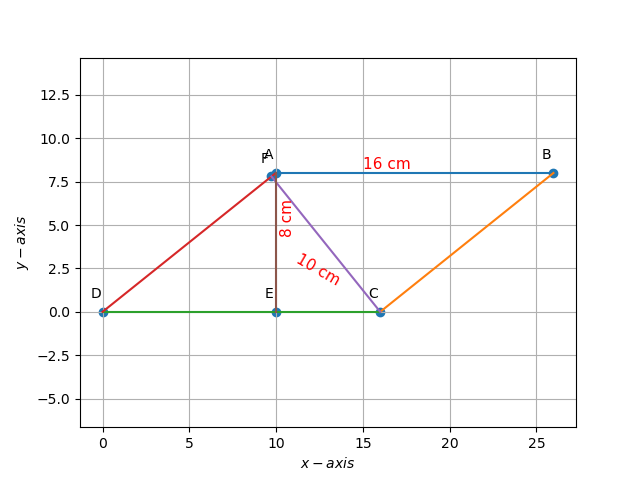
\includegraphics[width=\columnwidth]{chapters/9/10/4/figs/fig1.jpg}
    \caption{}
    \label{fig:chapters/9/10/41}
\end{figure}
\item Three girls Reshma, Salma and Mandip are playing a game by standing on 
a circle of radius 5m drawn in a park. Reshma throws a ball to Salma, Salma to 
Mandip, Mandip to Reshma. If the distance between Reshma and Salma and between 
Salma and Mandip is 6m each, what is the distance between Reshma and Mandip?
\\
\solution 
\input{chapters/9/10/4/5/circle.tex}
\item A circular park of radius 20m is situated in a colony. Three boys Ankur,
Syed and David are sitting at equal distance on its boundary each having a toy 
telephone in his hands to talk each other. Find the length of the string of each 
phone.
\item If two equal chords of a circle intersect within the circle, prove 
that the line joining the point of intersection to the centre makes equal 
angles with the chords.
\label{chapters/9/10/4/6}
%\label{chapters/9/10/4/6}
\\
\solution 
%\input{chapters/9/10/4/6/circle.tex}
\input{chapters/9/10/4/6/circle.tex}
\item  $\vec{A},\vec{B},\vec{C}$ are the three points on a circle with centre $\vec{O}$ such that $\angle$BOC=30\degree and $\angle$AOB=60\degree. If $\vec{D}$ is a point on the circle other than the arc ABC, find $\angle$ADC.
\label{chapters/9/10/5/1}
\\
\solution
\input{chapters/9/10/5/1/circle.tex}
\item A chord of a circle is equal to the radius of the circle. Find the angle subtended by the chord at a point on the minor arc and also at a point on the major arc.
\label{chapters/9/10/5/2}
\\
\solution
\input{chapters/9/10/5/2/circle.tex}

\item If diagonals of a cyclic quadrilateral are diameters of the circle through the vertices of quadrilateral,prove that it is a rectangle.\\
\label{chapters/9/10/5/7}
\solution
\input{chapters/9/10/5/7/circle.tex}
\item If circles are drawn taking two sides of a triangle as diameters, prove that the point of intersection of these circles lie on the third side.
\label{chapters/9/10/5/10}
\\
\solution
\input{chapters/9/10/5/10/circle.tex}
    \item Prove that a cyclic paralellogram is a rectangle.
\label{chapters/9/10/5/12}
\\
\solution
\input{chapters/9/10/5/12/circle.tex}
\item Prove that the line of centres of two intersecting circles subtends equal angles at the two points of intersection.
\\
    \solution 
\label{chapters/9/10/6/1}
\input{chapters/9/10/6/1/circle.tex}
\item  $AC$ and $BD$ are chords of a circle which bisect each other. Prove that 
	\begin{enumerate}
		\item  $AC$ and $BD$ are diameters, 
		\item  $ABCD$ is a rectangle.
	\end{enumerate}
    \solution 
\label{chapters/9/10/6/7}
\input{chapters/9/10/6/7/circle.tex}
\item Bisectors of angles $A,B$ and $C$ of a triangle $ABC$ intersect its circumcircle at $D,E$ and $F$ respectively. Prove that the angles of triangle $DEF$ are $90{\degree} - \frac{A}{2}$, $90{\degree}-\frac{B}{2}$ and $90{\degree} - \frac{C}{2}$.
\label{chapters/9/10/6/8}
\\
    \solution 
\input{chapters/9/10/6/8/circle.tex}
\item Two congruent circles intersect each other at points $\vec{A}$ and $\vec{B}$. Through $\vec{A}$ any line segment $\vec{PAQ}$ is drawn so that $\vec{P}$, $\vec{Q}$ lie on the two circles. Prove that $BP = BQ$.
\label{chapters/9/10/6/9}
\\
    \solution 
\input{chapters/9/10/6/9/circle.tex}
\item In any $\triangle ABC$, if the angle bisector of $\angle A$ and 
    perpendicular bisector of $BC$ intersect, prove that they intersect on 
    the circumcircle of $\triangle ABC$.
\\
    \solution 
\label{chapters/9/10/6/10}
\input{chapters/9/10/6/10/circle.tex}

\item
In \figref{fig:9.10.5.3.1} or,\figref{fig:9.10.5.3.2},$\angle PQR = 100\degree$,where $P,Q$ and $R$ are points on a circle with centre $O$.Find $\angle OPR$.

\textbf{Solution :}
\begin{table}[H]
    \centering
        \begin{tabular}{|c|c|c|}
    \hline
    \textbf{Input Parameters} &\textbf{Description} &\textbf{Value} \\
    \hline
     $\vec{O}$& Center(at origin)&$\vec{0}$\\
     \hline
 $r$ & Radius &1\\
 \hline
 $\theta$&$\angle PQR$&$100\degree$\\
 \hline
 $\theta_1$&$\angle NOQ $&$\theta_1\degree$\\
 \hline
 $\theta_2$&$\angle NOP $&$165\degree$\\
 \hline
 $\theta_3$&$\angle NOR $&$5\degree$\\
 \hline
  \end{tabular}

    \caption{Table of input parameters}
    \label{tab:9.10.5.3.1}
\end{table}

\begin{table}[H]
    \centering
        \begin{tabular}{|c|c|c|}
    \hline
        \textbf{Output Parameters} &\textbf{Description} &\textbf{Value} \\
\hline
          $\vec{Q}$ & Point &$\myvec{\cos{\theta_1}\\\sin{\theta_1}}$\\
          \hline
          $\vec{P}$ & Point &$\myvec{\cos{\theta_2}\\\sin{\theta_2}}$ \\
         \hline
          $\vec{R}$ & Point &$\myvec{\cos{\theta_3}\\sin{\theta_3}}$ \\
         \hline
    \end{tabular}

    \caption{Table of output parameters}
    \label{tab:9.10.5.3.2}
\end{table}

For getting the value of the $\angle NOQ$

\begin{align}
    \cos{\theta}&=\frac{\brak{\vec{R-Q}}^{\top}\brak{\vec{P-Q}}}{\vec{\norm{R-Q}\norm{P-Q}}}\\
    or,\cos{\theta}&=\frac{\sin{\frac{\theta_1+\theta_2}{2}}\cos{\frac{\theta_2+\theta_3}{2}}}{\sin{\frac{\theta_2-\theta_1}{2}}}\\
    so,\theta_1&=2\tan^{-1}\brak{\tan\brak{{\frac{\theta_2}{2}}}\brak{\frac{\cos{\theta}+\cos{\frac{\theta_2+\theta_3}{2}}}{\cos{\theta}-\cos{\frac{\theta_2+\theta_3}{2}}}}}\\
    \implies \theta_1&=136.696\degree\\
    or,\theta_1&=2\tan^{-1}\brak{\tan\brak{{\frac{\theta_2}{2}}}\brak{\frac{\cos{\theta}-\cos{\frac{\theta_2+\theta_3}{2}}}{\cos{\theta}+\cos{\frac{\theta_2+\theta_3}{2}}}}}\\
    \implies \theta_1&=175\degree\\
\end{align}
For getting the value of the $\angle OPR$
\begin{align}
    \angle OQP +\angle OQR &=\theta\\
    \angle QOR &=180-2\angle OQR,\brak{OQ=OR}\\
        \angle QOP &=180-2\angle OQP,\brak{OQ=OP}\\
        or,\angle POR &= 360-\brak{\angle QOP+\angle QOR}\\
        \implies \angle POR &= 2\brak{\angle OQP +\angle OQR}\\
        &=2\theta\\
    \angle POR +\angle ORP +\angle OPR &= 180\degree\\
    \angle POR +2\angle OPR&= 180\degree, \brak{OR=OP}\\
\angle OPR &= \frac{180\degree-2\theta}{2}\\
 \angle OPR &=-10\degree
 \end{align}


  \begin{figure}[H]                              
 \centering                          
 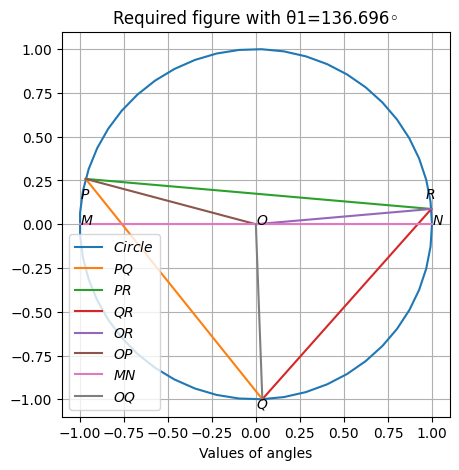
\includegraphics[width=\columnwidth]{chapters/9/10/5/3/fig/9.10.5.3.1.png}
\caption{}
	  \label{fig:9.10.5.3.1}
  \end{figure}
   \begin{figure}[H]                              
 \centering                          
 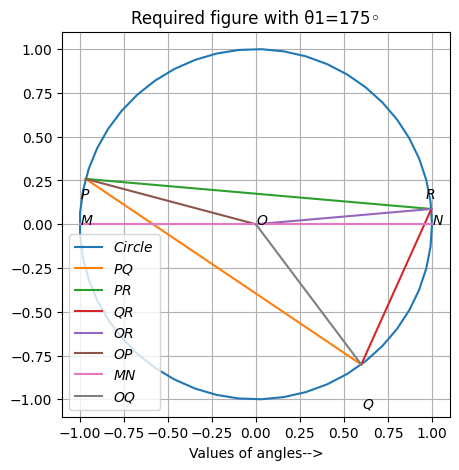
\includegraphics[width=\columnwidth]{chapters/9/10/5/3/fig/9.10.5.3.2.png}
\caption{}
	   \label{fig:9.10.5.3.2}
  \end{figure}

\item
If two equal chords of a circle intersect within the circle,prove that the line joining the point of intersection to the centre makes equal angles with the chords.

\textbf{Solution :}

\begin{table}[H]
    \centering
	 \begin{tabular}{|c|c|c|}
    \hline
    \textbf{Input Parameters} &\textbf{Description} &\textbf{Value} \\
    \hline
     $\vec{O}$& Center(at origin)&$\vec{0}$\\
     \hline
$d$&Length of the chords &2\\
 \hline
 $r$ & Radius &1\\
 \hline
 $\theta_1$&$\angle ROP$&$\theta_1\degree$\\
 \hline
 $\theta_2$&$\angle ROQ$&$-48\degree$\\
 \hline
 $\theta_3$&$\angle ROR $&$0\degree$\\
 \hline
 $\theta_4$&$\angle ROS $&$-132\degree$\\
 \hline
 
    \end{tabular}


    \caption{Table of input parameters}
    \label{tab:tab:9.10.4.3.1}
\end{table}

\begin{table}[H]
    \centering
\begin{tabular}{|c|c|c|}
    \hline
        \textbf{Output Parameters} &\textbf{Description} &\textbf{Value} \\
\hline
          $\vec{P}$ & Point &$\myvec{\cos{\theta_1}\\\sin{\theta_1}}$ \\

         \hline
          $\vec{Q}$ & Point &$\myvec{\cos{\theta_2}\\\sin{\theta_2}}$ \\
         \hline
          $\vec{R}$ & Point &$\myvec{\cos{\theta_3}\\\sin{\theta_3}}$ \\
         \hline
          $\vec{S}$ & Point &$\myvec{\cos{\theta_4}\\\sin{\theta_4}}$ \\
         \hline
    \end{tabular}


\caption{Table of output parameters}
    \label{tab:tab:9.10.4.3.2}
\end{table}

\begin{align}
  \cos{\angle RQS}&=\frac{\vec{\brak{R-Q}}^{\top}\vec{\brak{Q-S}}}{\vec{\norm{R-Q}\norm{Q-S}}}\\
  &=\cos{\frac{\theta_3-\theta_4}{2}}\\
   \cos{\angle PSQ}&=\frac{\vec{\brak{P-S}}^{\top}\vec{\brak{S-Q}}}{\vec{\norm{P-S}\norm{S-Q}}}\\
  &=\cos{\frac{\theta_1-\theta_2}{2}}\\
   \cos{\angle RQS}&=\cos{\angle PSQ}\\
   or,\theta_1&=\theta_2-\theta_3+\theta_4\\
   &=-180\degree
  \end{align}
The equation of $PQ$ and $RS$ is obtained by
\begin{align}
  \vec{n_1}^{\top}\vec{\brak{x-P}}=0\\
  \vec{n_2}^{\top}\vec{\brak{x-R}}=0\\
  or,\vec{n_1}=\myvec{\sin{\theta_2}-\sin{\theta_1}\\\cos{\theta_1}-\cos{\theta_2}}\\
  or,\vec{n_2}=\myvec{\sin{\theta_4}-\sin{\theta_3}\\\cos{\theta_3}-\cos{\theta_4}}\\
 \end{align}
  The value of the point of the intersection is
\begin{align}
    \myvec{\vec{n_1}^{\top}\\\vec{n_2}^{\top}}\vec{x}&=\myvec{\vec{n_1}^{\top}\vec{P}\\\vec{n_2}^{\top}\vec{R}}\\
    \vec{x}&=\myvec{\vec{n_1}^{\top}\\\vec{n_2}^{\top}}^{-1}\myvec{\vec{n_1}^{\top}\vec{P}\\\vec{n_2}^{\top}\vec{R}}\\
        or,\vec{T} &= \myvec{0\\-0.45}\\
\cos{\angle OTP} &= \frac{\brak{\vec{T-P}}^{\top}\brak{\vec{O-T}}}{\vec{\norm{T-P}\norm{T-O}}}\\
or, \angle OTP&= 66\degree
\end{align}
Similarly,
\begin{align}
   \cos{\angle OTR} &= \frac{\brak{\vec{T-R}}^{\top}\brak{\vec{T-O}}}{\vec{\norm{T-R}\norm{T-O}}}\\
or, \angle OTR&= 66\degree \\
So,\angle OTP &= \angle OTR \brak{proved}
\end{align}

 

\begin{figure}[H]                            
\centering
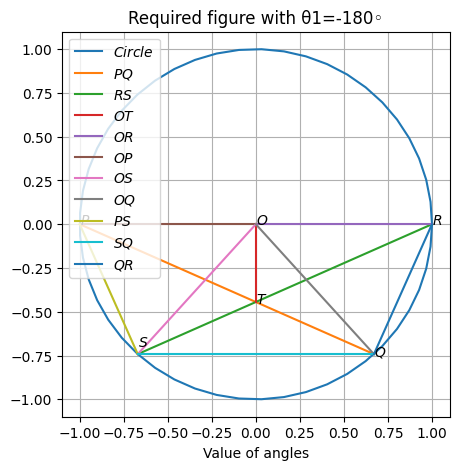
\includegraphics[width=\columnwidth]{chapters/9/10/4/3/fig/9.10.4.3.png}                            
\caption{}                              
\label{fig:9.10.4.3}
\end{figure}


\end{enumerate}
